\documentclass[a4paper]{article}

%% Language and font encodings
\usepackage[utf8]{inputenc}
\usepackage[ngerman]{babel}
\usepackage[T1]{fontenc}
\usepackage{caption}
\usepackage{enumitem}

%% Sets page size and margins
\usepackage[a4paper,top=3cm,bottom=2cm,left=3cm,right=3cm,marginparwidth=1.75cm]{geometry}

%% Useful packages
\usepackage{amsmath}
\usepackage{graphicx}
\usepackage[style=nature]{biblatex}
\usepackage[colorinlistoftodos]{todonotes}
\usepackage[colorlinks=true, allcolors=blue]{hyperref}
\usepackage{float}

% für tabellen
\usepackage{booktabs}

% für Gradzeichen
\usepackage{siunitx}

\addbibresource{references.bib}

\title{Praktikum Neurobiologie - Protokoll 5}

\author{Cedric Laier, Tilman Mehl}


\begin{document}
%Titelpage Modell: https://www.latextemplates.com/template/formal-book-title-page
\begin{titlepage} % Suppresses headers and footers on the title page

	\centering % Centre everything on the title page
	
	\scshape % Use small caps for all text on the title page
	
	\vspace*{\baselineskip} % White space at the top of the page
	
	%------------------------------------------------
	%	Title
	%------------------------------------------------
	
	\rule{\textwidth}{1.6pt}\vspace*{-\baselineskip}\vspace*{2pt} % Thick horizontal rule
	\rule{\textwidth}{0.4pt} % Thin horizontal rule
%	{\LARGE THE BIG BOOK\\ OF\\ \LaTeX ~TEMPLATES\\} % Title
	\vspace{0.75\baselineskip} % Whitespace above the title
	{\LARGE Psychophysische Experimente zum Farbensehen} {\\Protokoll zum Praktikum Neurobiologie für Bioinformatiker\\ am 04.02.2019} % Title

	
	\vspace{0.75\baselineskip} % Whitespace below the title
	
	\rule{\textwidth}{0.4pt}\vspace*{-\baselineskip}\vspace{3.2pt} % Thin horizontal rule
	\rule{\textwidth}{1.6pt} % Thick horizontal rule
	
	\vspace{2\baselineskip} % Whitespace after the title block
	
	\vspace{2.0\baselineskip} % Whitespace before the editors

{\LARGE Gruppe 2}
\vspace{2.5\baselineskip} \\
	
{\LARGE Autoren:}
\begin{itemize}
\item Cedric Laier - \textit{cedric.laier@fu-berlin.de}
\item Tilman Mehl - \textit{tilmanmehl@zedat.fu-berlin.de}
\end{itemize}
\vspace{2.5\baselineskip}

{\LARGE Lehrveranstalter:}
\begin{itemize}
\item  Peter Robin Hiesinger
\item Matthias Wernet
\end{itemize}
\vspace{2.5\baselineskip}

{\LARGE Tutoren:}
\begin{itemize}
\item Lisa
\item Johannes
\item Claudia
\end{itemize}
	
\end{titlepage}

%%
%%
%% Kapitel 1: Einleitung
%%
%%

\section{Einleitung}

Im Rahmen des 5. Praktikumstages behandelten wir die subjektive Wahrnehmung des menschlichen Farbensehens und untersuchten wie diese mit den messbaren physikalischen Reizen zusammenhängen.
%% Aufbau der menschlichen Retina. Zapfen, Stäbchen, wahrgenommene Wellenlängen
%% Additive und Subtraktive Farbmischung
%% Verdrahtung im Hirn (Adaption, laterale Inhibition, On/Off Verschaltung,...)


%%
%%
%% Kapitel 2: Versuchsaufbau- und durchführung
%%
%%

\section{Versuchsaufbau und -durchführung}

\subsection{Fragen im Skript}

Für diese Experiment Aufgabe war kein Aufbau nötig, die Antworten finden sich unter Kapitel 3.1.

\subsection{Farbenkreis}

Auf den Computern die für den Praktikumstag bereitgestellt wurden, befand sich ein Anwendung mit dem Namen \texttt{farbkreis.bat}. Nach dem Ausführen der Datei wurden uns auf dem Bildschirm in einem weißen Bildschirmfenster mehrere unterschiedliche Farbstimuli (Farbkreise) zufällig verteilt angezeigt. Ziel war es mit der Computer Maus die Farbstimuli in einem Kreis anzuordnen. Wir haben dabei mit dem roten Farbstimuli begonnen und systematisch alle Farben verglichen (heller, dunkler oder farbähnlich) relativ intuitiv kreisförmig angeordnet. Unserer Resultat ist in Abbildung \ref{fig:A2a} im Kapitel 3.2  zu sehen.

\subsection{Farbmischung}

Hier wurde ein Programm mit dem Namen \texttt{rgbmon.bat} gestartet. Mithilfe dieses Programmes waren wir in der Lage den drei RGB Grundfarben (Rot, Grün und Blau) jeweils einzele Farmischungswerte von 0\% - 100\% des Monitors einzustellen. Durch das Verstellen der einzelnen Regler konnten wir somit neue Farmischungen erzeugen.

\subsection{Farbintensität}

Bei der vierten Aufgabe benötigten wir das Programm \texttt{ipxl.bat}. Über den Menüpunkt "Select" wählten wir unter dem Reiter ''Experiments'' das ''Simple colored disk'' Experiment aus. Zusätzlich haben wir über den Menüpunkt "Options" die Option für ''Follow invalid colors'' deaktiviert. \\

\noindent Über das Setzen der Haken für Yxy und L*a*b Farbraum unter "Systems" konnten wir uns nun auch noch die Koordinaten für die unterschiedlichen Koordinaten anzeigen lassen. 

\noindent In diesem Experiment wurden folgende Eigenschaften geändert und beobachtet:

\begin{itemize}
    \item Justierung der Intensität
    \item Veränderung des Farbtons, Sättigung, Helligkeit des Farbstimulus.
    \item Verminderung der Sättigung bei konstanter Intensität
    \item Wahl verschiedener Intensitäten des Stimulus
    \item Veränderung des Hintergrunds vom Farbstimulus von dunkel zu hell
\end{itemize}

\noindent Die Beobachtungen und Ergebnisse zum Experiment mit \texttt{IPXL} befinden sich im Kapitel 3.4.

\newpage
\subsection{Farbenreihe}
Für diesen Versuch wurde mit IPXL die Anwendung "High intensity stairs: Contrast" (unter Select -> Test displays) gestartet. Es wurden drei Farbenreihen erstellt, bei denen sich jeweils eine Eigenschaft schrittweise ändert (und die anderen beiden Eigenschaften gleich bleiben):
\begin{itemize}
    \item Änderung des Farbtons
    \item Änderung der Helligkeit
    \item Änderung der Sättigung
\end{itemize}
Um die Änderung des Farbtons zu erreichen wurde für den ersten Balken eine Startfarbe gewählt. Dann wurden für die anderen Balken gegen den Uhrzeigersinn sechs weitere Punkte kreisförmig um den Weißpunkt ausgewählt.\\
Für die Änderung der Helligkeit wurde ein Startpunkt gewählt, und der Helligkeitsregler auf 80 gestellt. Für die anderen Balken wurde der Helligkeitsregler schrittweise reduziert.\\
Für die Änderung der Sättigung wurde ein Startpunkt nahe dem Weißpunkt gewählt. Dann wurden auf einer Linie zwischen Weißpunkt und Dreiecksrand Punkte gewählt, und den anderen Balken zugewiesen.

\subsection{Farbmischung}
Für diesen Versuch wurde mit IPXL die Anwendung 'Matching and Spatial mixture' (unter Select -> Photometry and Mixture) gestartet. Zunächst wurde für das linke Viereck eine neue Farbe bestimmt. Anschliessend wurden für das rechte Viereck zwei Farben ermittelt, die durch additive Farbmischung die beiden Vierecke farblich gleich aussehen lassen.\\
Der Versuch wurde auch noch für ein weiteres Paar an Farben durchgeführt.

\subsection{Simultaner Farbkontrast}
Für diesen Versuch wurde mit IPXL die Anwendung 'Simultaneous color contrast' (unter Select -> Simple contrast effects) gestartet. Dabei sind zwei Vierecke zu sehen, die mit andersfarbigen Vierecken umrandet sind.  Mit dem Button 'Step' wurde die Umrandung entfernt, und die jeweiligen Sinneseindrücke protokolliert.\\
Für die verschiedenen Vierecke wurden unterschiedliche Farbkombination probiert, um die inneren Vierecke möglichst unterschiedlich erscheinen zu lassen.

\subsection{Sukzessiver Farbkontrast}
Für diesen Versuch wurden mit IPXL jeweils die Anwendungen 'Aftereffects and Opponent Colors', 'Induction', 'Desaturation by Adaptation' und 'Hypersaturation' gestartet (jeweils unter Select -> Adaptation effects).\\
Für die Durchführung wurde der Blick jeweils 30 Sekunden auf den Bildmittelpunkt fixiert, und dann der Button 'Step' gedrückt (2 mal für "Hypersaturation"). Die erscheinenden Nachbilder wurden protokolliert.

%%
%%
%% Kapitel 3: Ergebnisse
%%
%%

\newpage
\section{Ergebnisse}
\subsection{Fragen im Skript}
\vspace{1.5\baselineskip}

\textbf{Der Spektralfarbenzug ist konvex gekrümmt. (Warum ist das so?)} \\

\noindent A: Der Spektralfarbenzug ist konvex gekrümmt in allen Farbebenen, weil die entsprechenden Rezeptoren in diesem Bereich noch angeregt sind. Punkte außerhalb der Kurvenzugs entsprechen keiner für uns sichtbaren Farbe.

\vspace{1.0\baselineskip}

\noindent\textbf{Warum liegen die Farborte von spektral breitbandigen Lichtern stets innerhalb des Spektralfarbenzugs?} 

\vspace{1.0\baselineskip}

\noindent A: Von spektral breitbandig spricht man bei Mischungen aus versch. Farben, die demzufolge nicht vollständig gesättigt sind. Sie können daher nur innerhalb des Spektralfarbenzugs liegen. \\

\vspace{1.0\baselineskip}

\noindent\textbf{Warum lässt sich aus solchen breitbandigen Lichtern nicht jede Farbe mischen (welche nicht?)?} 

\vspace{1.0\baselineskip}
\noindent A: Sie sind keine Grundfarben und nur diese können alle anderen Farben additiv mischen. Es lassen sich keine monochromatischen Farben (wie Blau, Rot etc.) mischen.

\newpage
\subsection{Farbenkreis}
\vspace{2.5\baselineskip}
\begin{figure}[H]
    \centering
    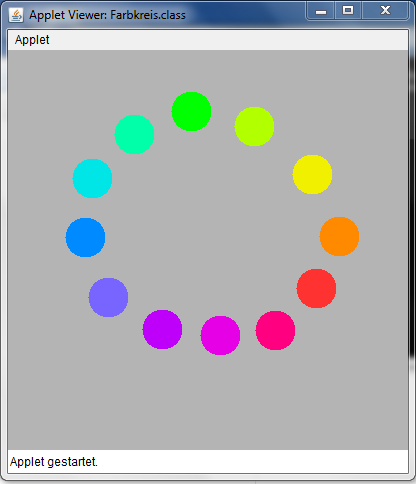
\includegraphics[width=0.5\columnwidth]{images/A2_Farbkreis.PNG}
    \caption{Unsere Anordnung des Farbenkreis}
    \label{fig:A2a}
\end{figure}
\vspace{2.5\baselineskip}
\begin{figure}[H]
    \centering
    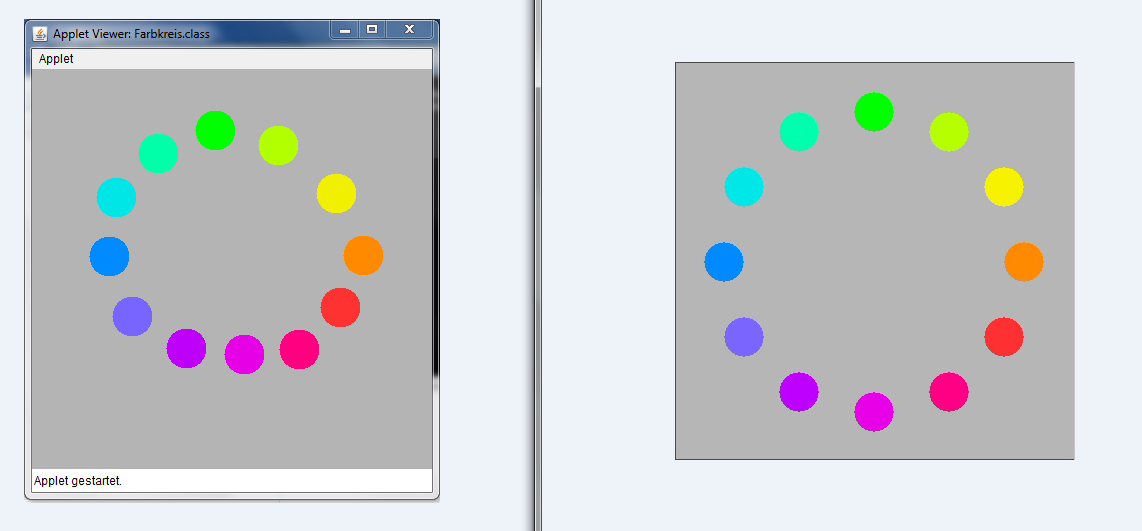
\includegraphics[width=0.9\columnwidth]{images/A2_FarbkreisFertigVergleich.PNG}
    \caption{links: Zum Vergleich unser Farbkreis (links) und der Musterfarbkreis (rechts)}
    \label{fig:A2b}
\end{figure}

\newpage
\subsection{Farmischung I}

\begin{figure}[H]
    \centering
    \begin{minipage}[b]{0.45\textwidth}
    	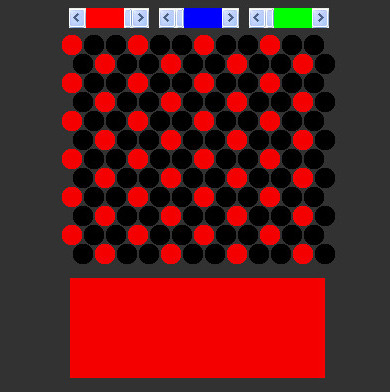
\includegraphics[width=0.9\columnwidth]{images/A3_rot.jpg}
    	\centering
    	\caption{Farbmischung Rot}
    	\label{fig:a3_rot}
    \end{minipage}
    \hfill
    \begin{minipage}[b]{0.45\textwidth}
    	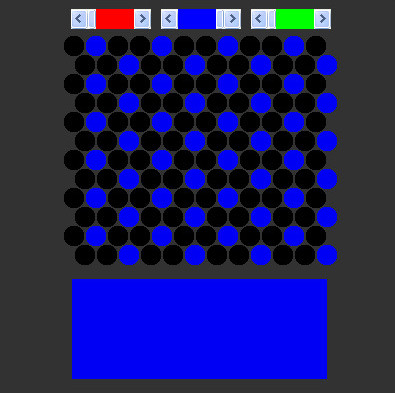
\includegraphics[width=0.9\columnwidth]{images/A3_blau.jpg}
    	\centering
    	\caption{Farbmischung Blau}
    	\label{fig:a3_blau}
    \end{minipage}
\end{figure}

In Abbildung \ref{fig:a3_rot} \& \ref{fig:a3_blau} ist zu sehen, dass wir die jeweiligen Farben erzeugt haben, indem wir den Farbanteil der anderen beiden auf 0 gesetzt haben. Daher spricht man hier von monochronmatischen Farben, welche nicht durch eine additive Mischung entstehen.

\vspace{2.5\baselineskip}
\begin{figure}[H]
    \centering
    \begin{minipage}[b]{0.45\textwidth}
    	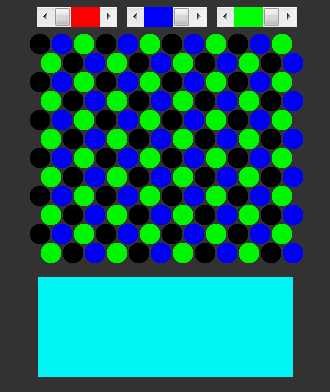
\includegraphics[width=0.9\columnwidth]{images/A3_cyan.PNG}
    	\centering
    	\caption{Farbmischung Cyan}
    	\label{fig:a3_cyan}
    \end{minipage}
    \hfill
    \begin{minipage}[b]{0.45\textwidth}
    	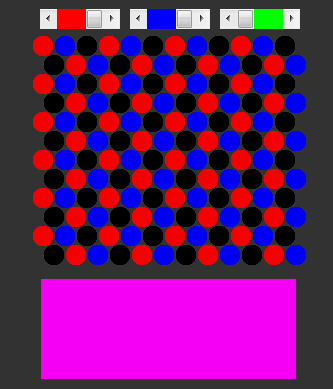
\includegraphics[width=0.9\columnwidth]{images/A3_magenta.PNG}
    	\centering
    	\caption{Farbmischung Magenta}
    	\label{fig:a3_magenta}
    \end{minipage}
\end{figure}

\noindent Die Farbmischungen in Abbildung \ref{fig:a3_cyan} \& \ref{fig:a3_magenta} haben wir erzeugen können, indem wir jeweils zwei der drei Farbregler aufs Maximum und den dritten auf 0 gestellt haben. Die Farmischung in Abbildung \ref{fig:a3_cyan} wurde aus den Grundfarben Grün und Blau erzeugt. Das Magenta in Abbildung \ref{fig:a3_magenta} konnten aus den Farben Rot und Grün gemischt werden.

\begin{figure}[H]
    \centering
    \begin{minipage}[b]{0.45\textwidth}
    	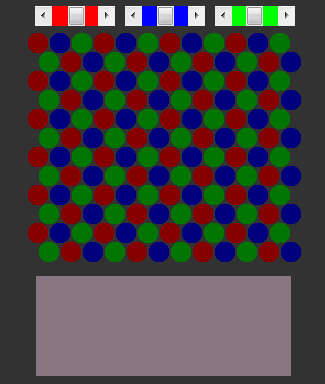
\includegraphics[width=0.89\columnwidth]{images/A3_grau.PNG}
    	\caption{Farbmischung Grau}
    	\centering
    	\label{fig:a3_grau}
    \end{minipage}
    \hfill
    \begin{minipage}[b]{0.45\textwidth}
    	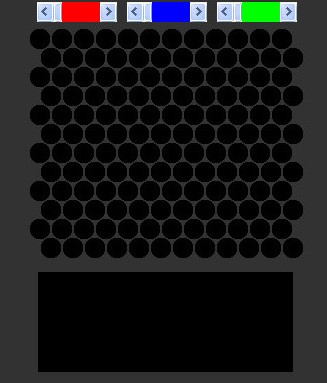
\includegraphics[width=0.9\columnwidth]{images/A3_schwarz.jpg}
    	\centering
    	\caption{Farbmischung Schwarz}
    	\label{fig:a3_schwarz}
    \end{minipage}
    \hfill
\end{figure}

\noindent Die Töne Schwarz und Weiss konnten erzeugt werden, indem sämtliche Farben auf 0\% bzw. 100\% geschaltet wurden. Das Schwarz wie es in Abbildung \ref{fig:a3_schwarz} zu sehen ist, ist enstanden indem wir alle drei Farbregler auf 0 gesetzt haben. \\ \\

\noindent Im Experiment haben wir das Prinzip der additiven Farmmischungen behandelt und wir konnten demonstrieren, dass mit den monochromatischen Grundfarben viele weitere Farben, Graustufen, Schwarz und Weiß erzeugt werden können.

\newpage
\subsection{Farbintensität}

\subsubsection*{a)}

\begin{figure}[H]
    \centering
    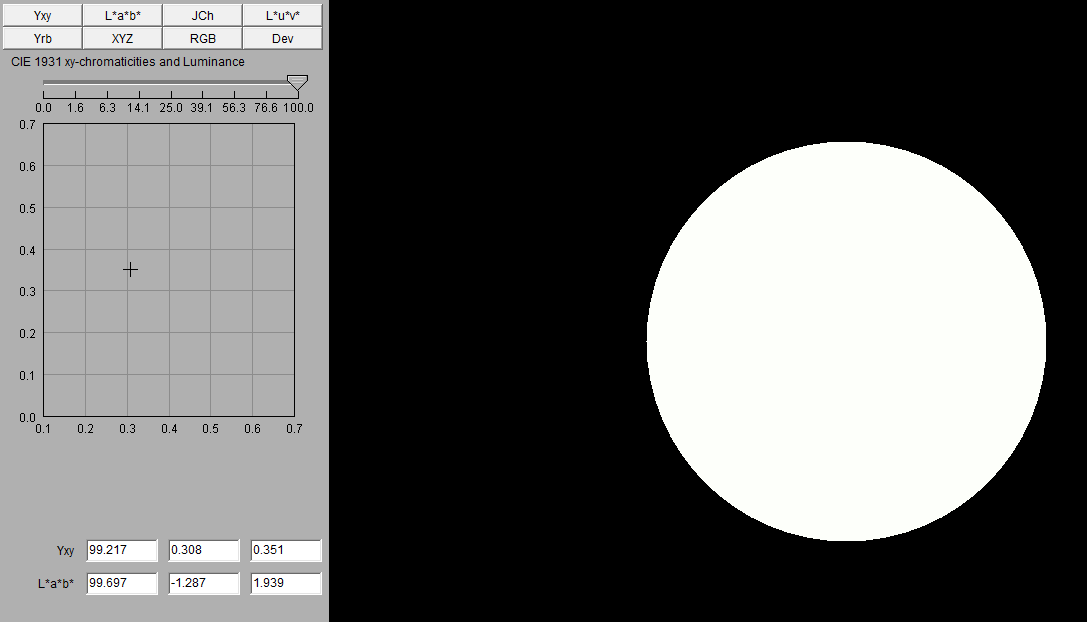
\includegraphics[width=0.8\columnwidth]{images/A4_a_Weisspunkt.PNG}
    \caption{Unser Weißpunkt im Farbraum}
    \label{fig:A3a}
\end{figure}

Der Weißpunt (wie in Abbildung \ref{fig:A3a} zu sehen) an dem Punkt an dem der Anteil aller Grundfarben gleich groß ist. Die Koordinaten sind in unserem Fall für Yxy \texttt{(99.217,0.308,0.351)} und bei L*a*b* \texttt{(99.697,-1.287,1.939)}.

\subsubsection*{b)}

\begin{figure}[H]
    \centering
    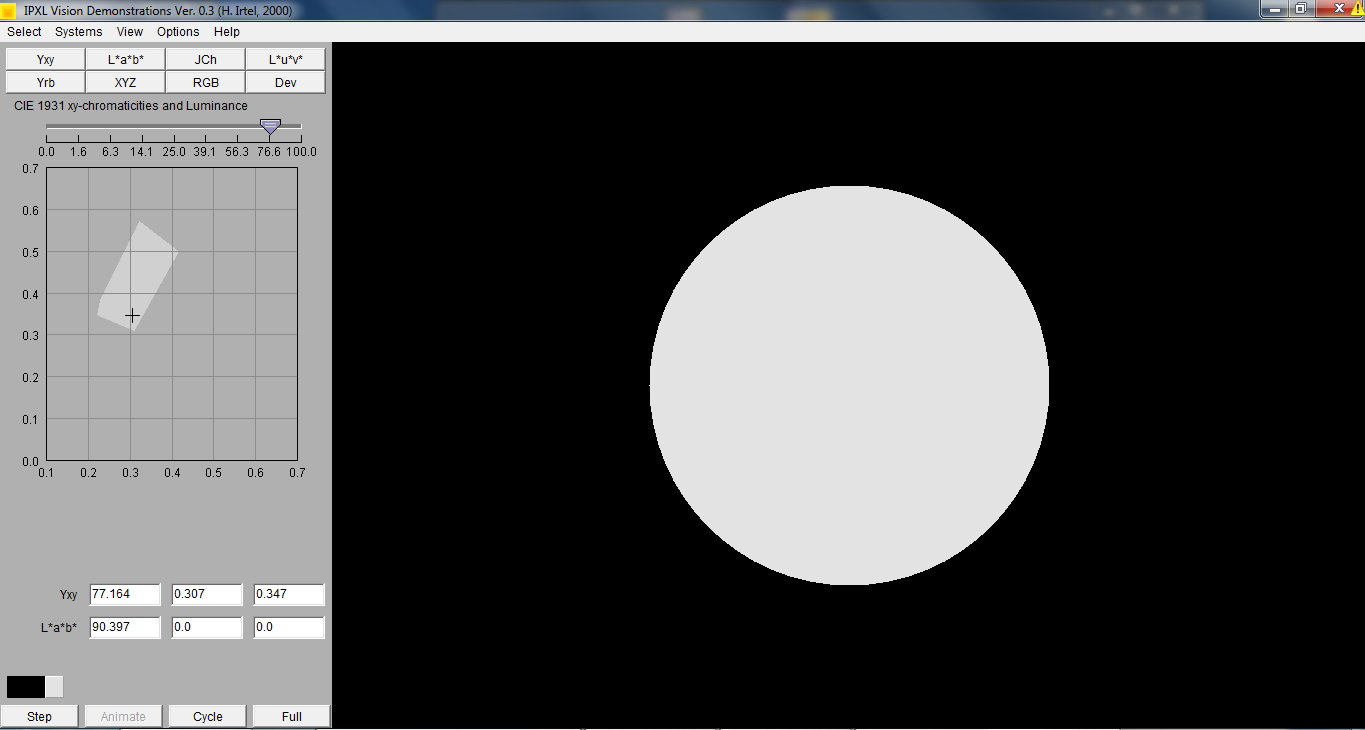
\includegraphics[width=0.8\columnwidth]{images/A4_b_Veraenderung_der_Intensitaet}
    \caption{Der Weißpunkt bei reduzierter Intensität/Helligkeit}
    \label{fig:A3b}
\end{figure}

Bei einer reduzierten Intensität wie in Abbildung \ref{fig:A3b} wirkt der Weißpunkt weniger hell und treibt dabei gleichzeitig ins Gräuliche ab.

\newpage
\subsubsection*{c, d \& e)}

\begin{figure}[H]
    \centering
    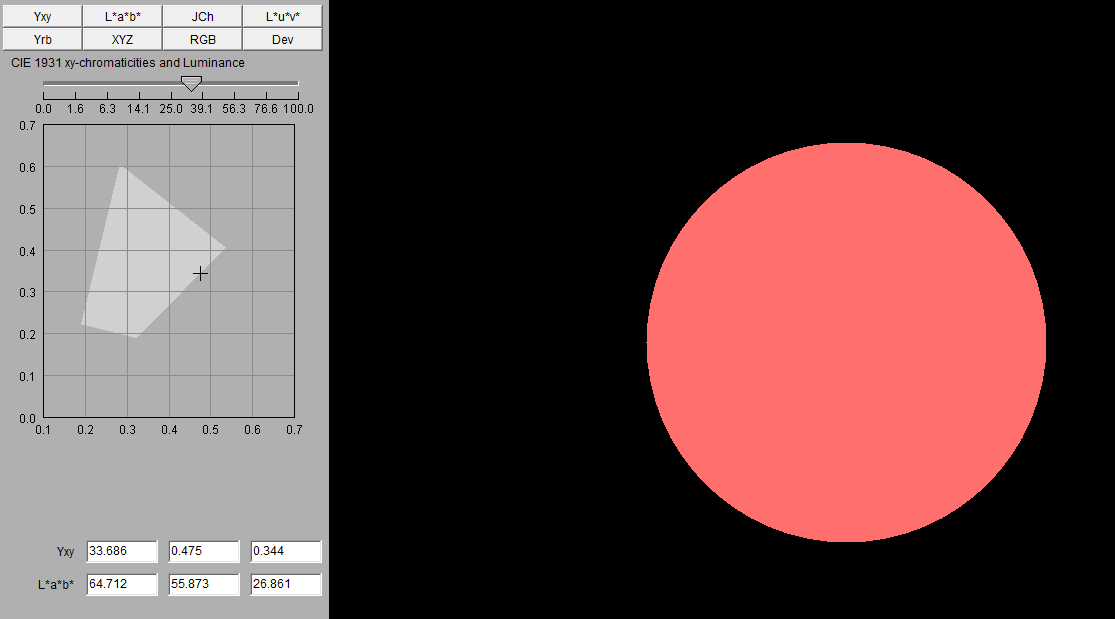
\includegraphics[width=0.7\columnwidth]{images/A4_cde_BlassesHellesRot.PNG}
    \caption{Blasses helles Rot}
    \label{fig:A4cde1}
\end{figure}

\begin{figure}[H]
    \centering
    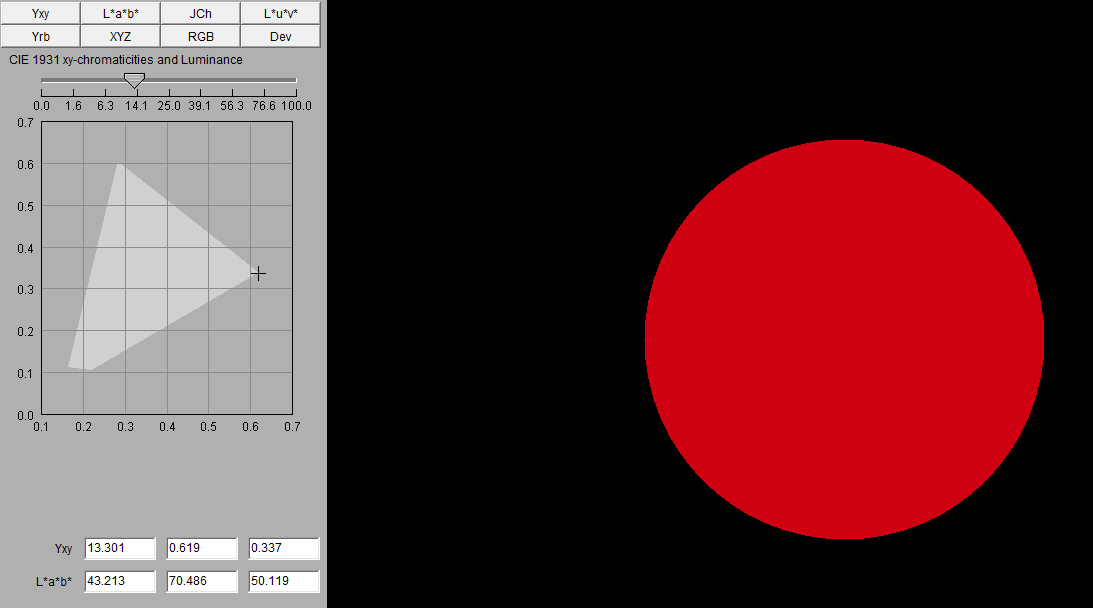
\includegraphics[width=0.7\columnwidth]{images/A4_cde_SattesRot.PNG}
    \caption{Sattes Rot}
    \label{fig:A4cde2}
\end{figure}

\begin{figure}[H]
    \centering
    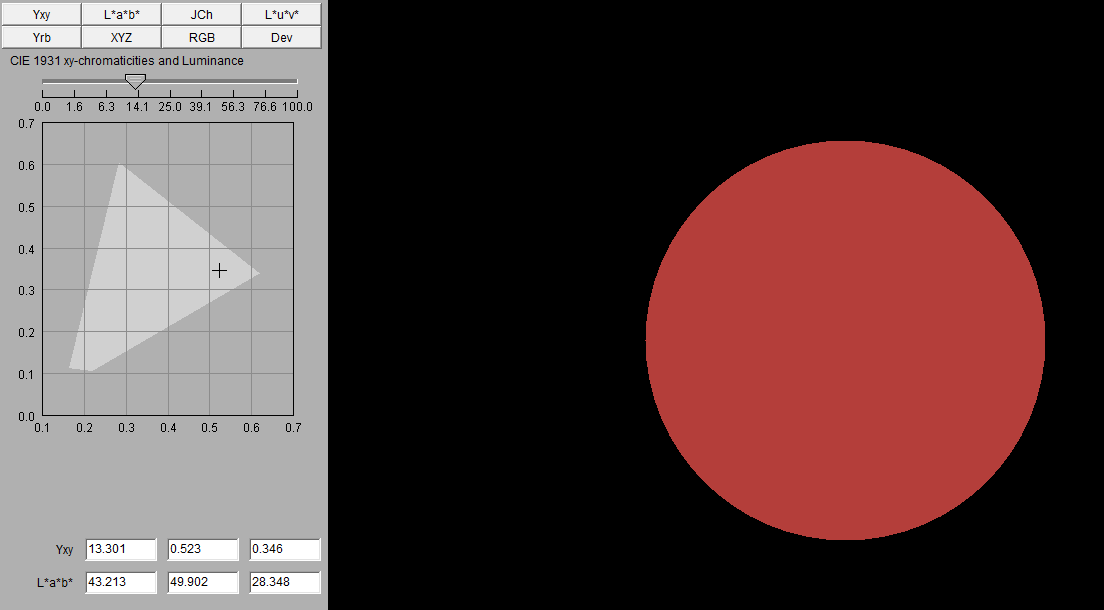
\includegraphics[width=0.7\columnwidth]{images/A4_cde_BlassesRot.PNG}
    \caption{Blasses Rot}
    \label{fig:A4cde3}
\end{figure}

Abbildung \ref{fig:A4cde2} und \ref{fig:A4cde3} unterscheiden sich nur bei dem Wert der Sättigung. Diese ist bei Abb. \ref{fig:A4cde3} vermindert, wodurch Abb. \ref{fig:A4cde3} weniger bunt wirkt. 

\begin{figure}[H]
    \centering
    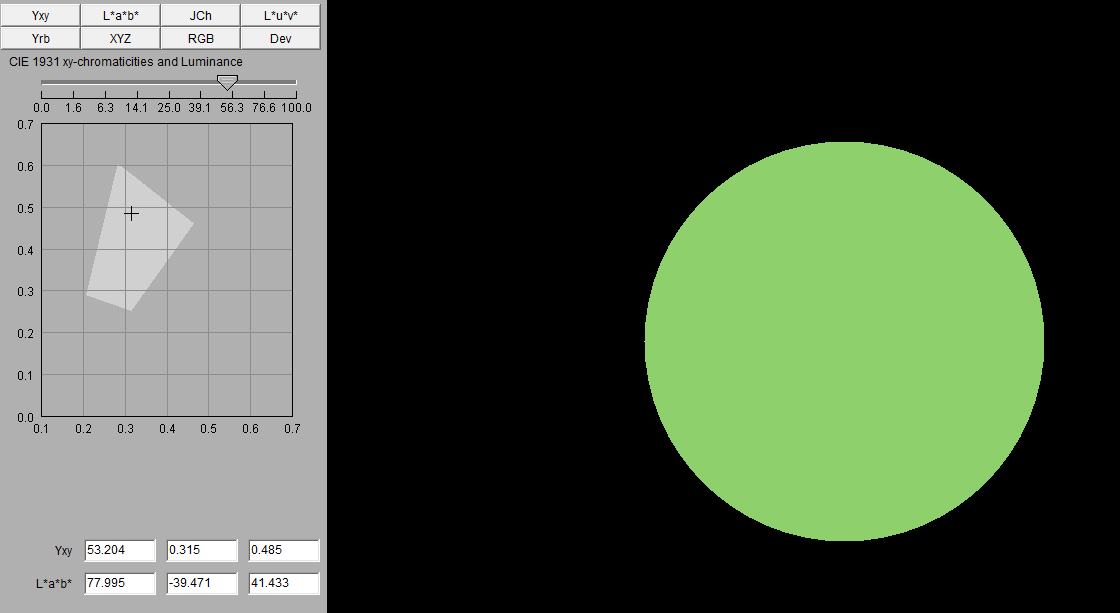
\includegraphics[width=0.7\columnwidth]{images/A4_cde_BlassesHellesGruen.PNG}
    \caption{Blasses helles Grün}
    \label{fig:A4cde4}
\end{figure}

\noindent Wie in Abbildung \ref{fig:A4cde4} zu sehen ist, wirkt die Farbe bei geringerer Sättigung etwas gräulicher. Um die Sättigung bei gleichbleibender Helligkeit zu verringern, mussten wir dem Spektralfarbzug ein Stück ins Zentrum folgen.

\begin{figure}[H]
    \centering
    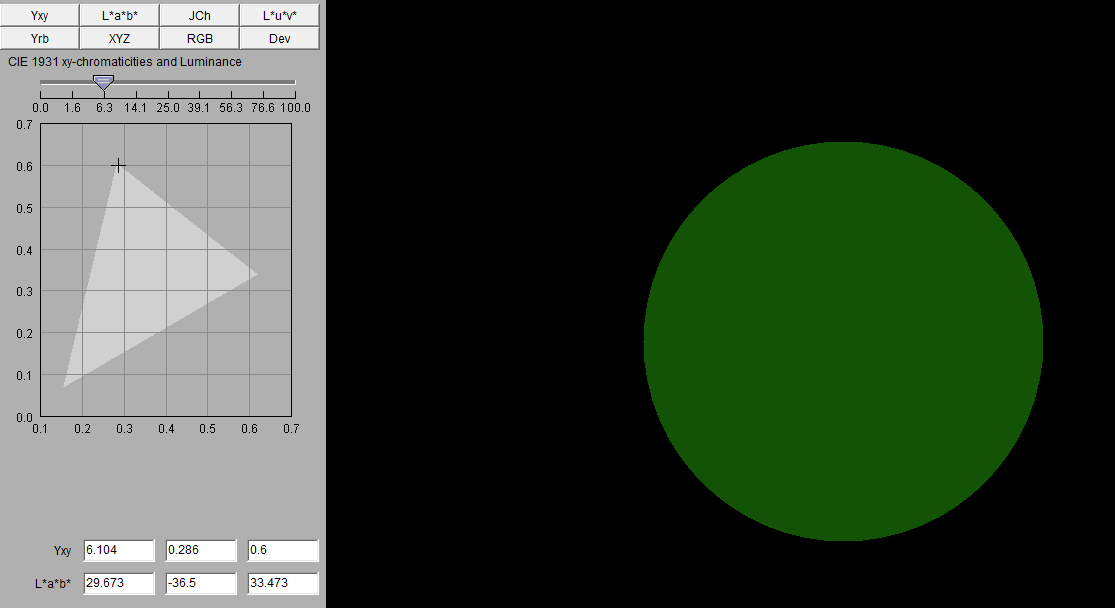
\includegraphics[width=0.7\columnwidth]{images/A4_cde_DunklesSattesGruen}
    \caption{Dunkles, sattes Grün bei geringer Intensität}
    \label{fig:A4cde5}
\end{figure}

\begin{figure}[H]
    \centering
    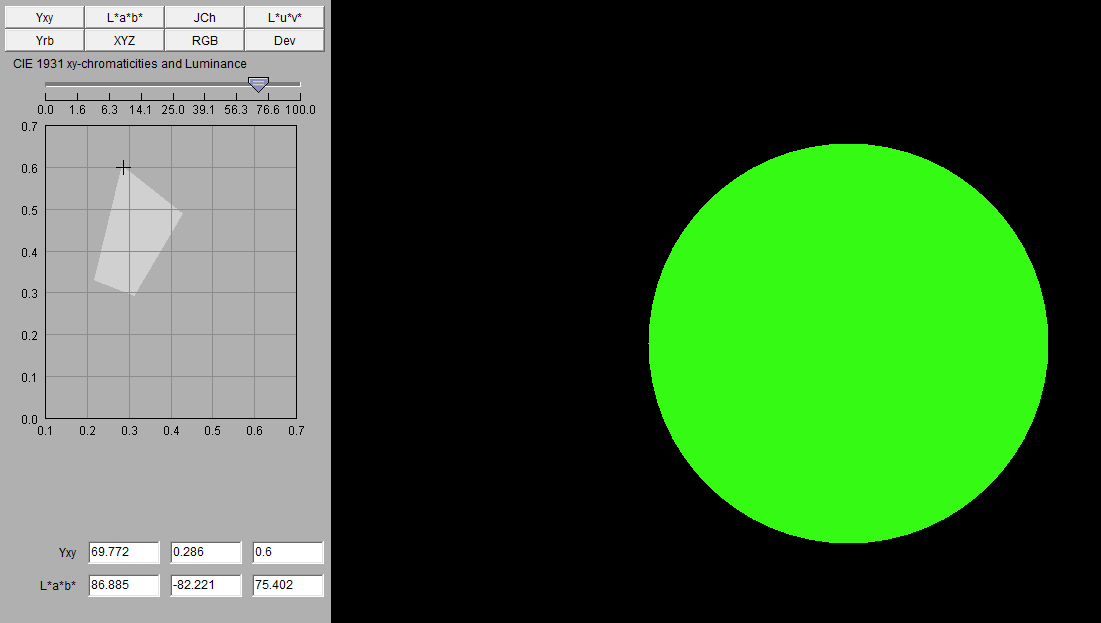
\includegraphics[width=0.7\columnwidth]{images/A4_cde_SattesGruen.PNG}
    \caption{Sattes Grün, hohe Sättigung und hohe Helligkeit des Farbtons}
    \label{fig:A4cde6}
\end{figure}

\subsubsection*{f)}

\begin{figure}[H]
    \centering
    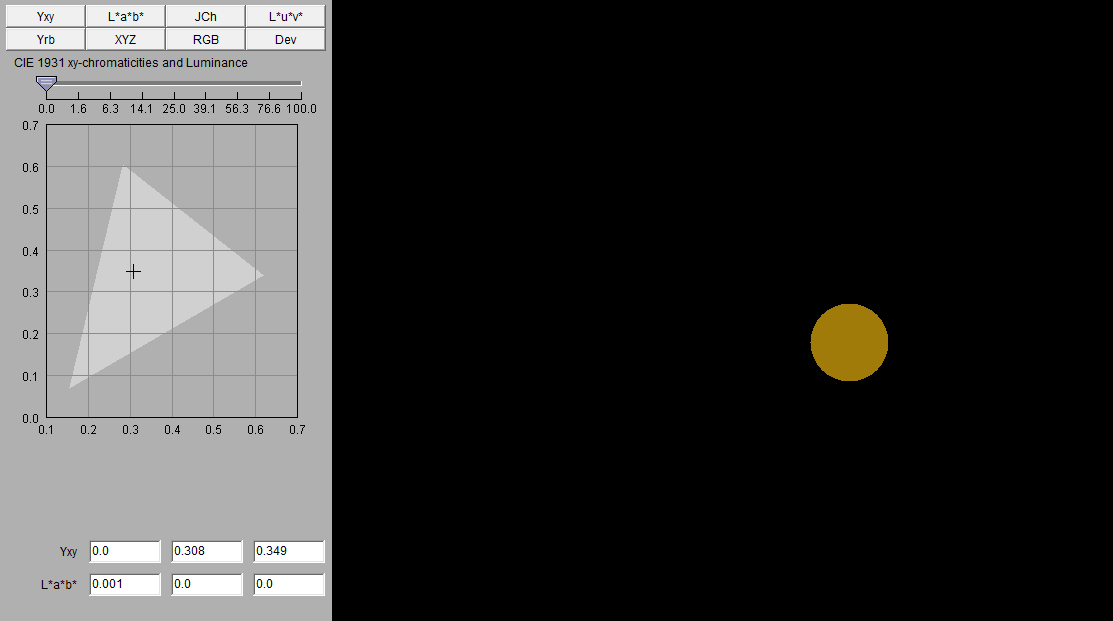
\includegraphics[width=0.9\columnwidth]{images/A4_f_DunklerHintergrundSmall.PNG}
    \caption{Kleine Farbfläche bei schwarzem Hintergrund}
    \label{fig:A4f}
\end{figure}

\begin{figure}[H]
    \centering
    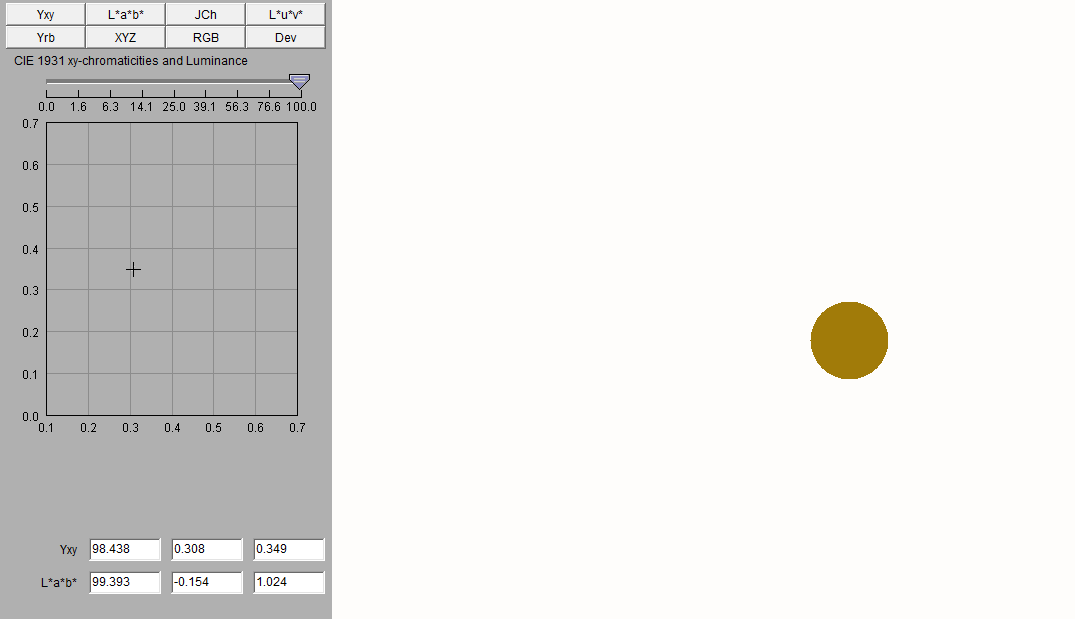
\includegraphics[width=0.9\columnwidth]{images/A4_f_HellerHintergrundSmall.PNG}
    \caption{Farbfläche bei weißem Hintergrund}
    \label{fig:A4f2}
\end{figure}

Bei einem direktem Vergleich von Abbildung \ref{fig:A4f} und Abbildung \ref{fig:A4f2} konnte man im Experiment feststellen, dass ein dunkler Hintergrund die Farbe heller wirken lässt und ein heller Hintergrund den Farbpunkt dunkler wirken lässt. \\ \\
Ein kleiner Stimulus (in unserem Falle der Farbkreis) verstärkt diesen Effekt (Simultan-Kontrast\footnote{\url{https://de.wikipedia.org/wiki/Sieben_Farbkontraste#Simultankontrast}}) noch einmal. 

\newpage
\subsection{Farbenreihe}
Die Farbenreihen sind in den Abbildungen \ref{fig:A5a}, \ref{fig:A5b}, und \ref{fig:A5c} dargestellt.
\begin{figure}[H]
    \centering
    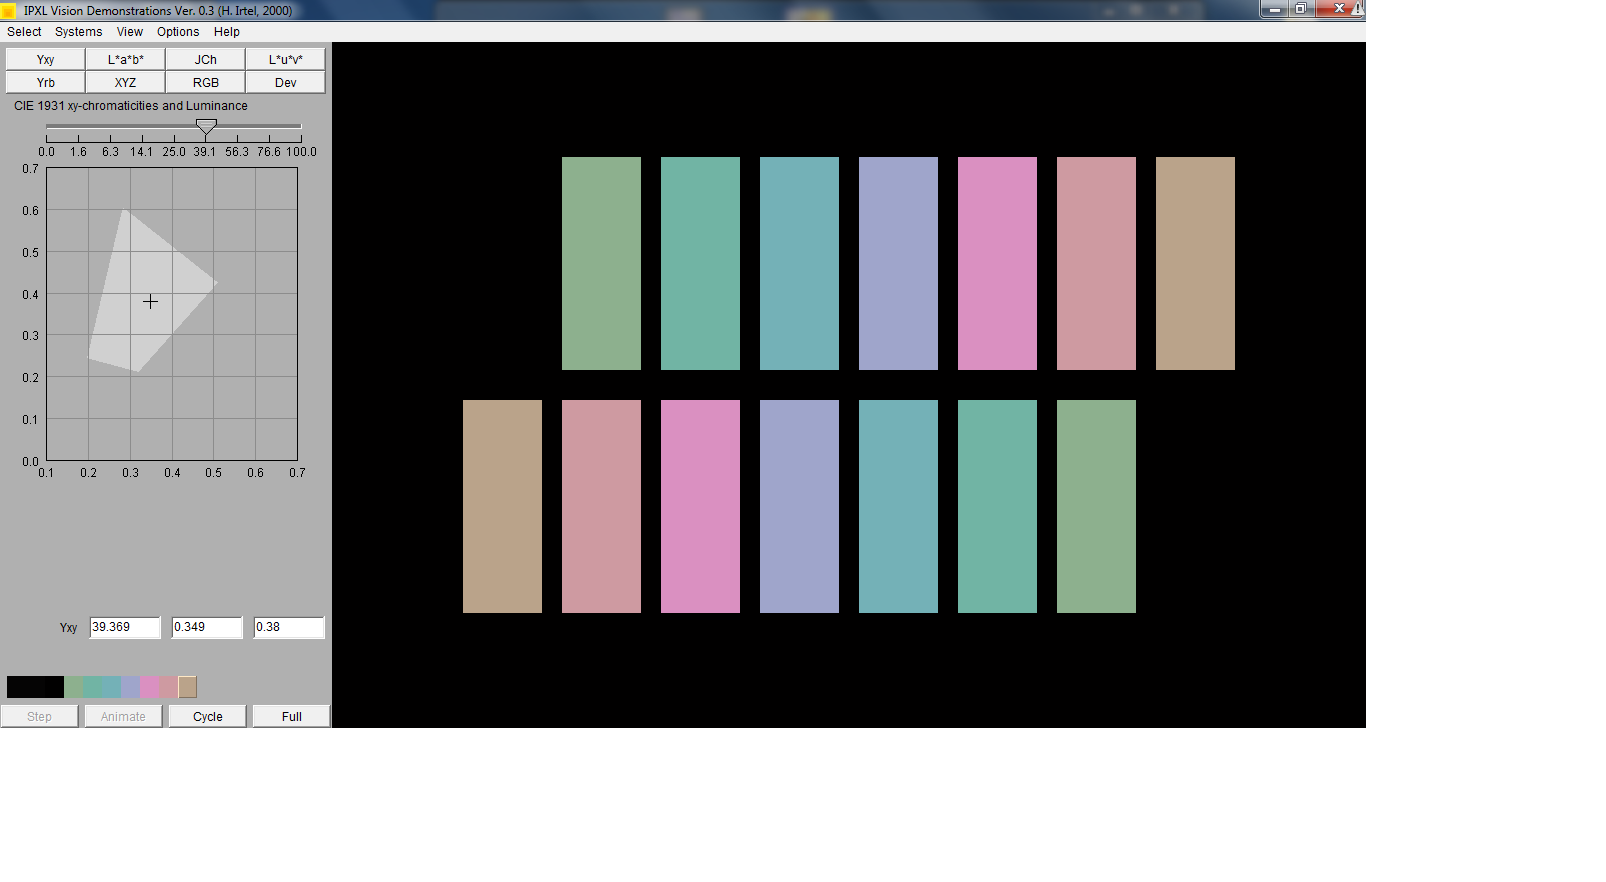
\includegraphics[width=\textwidth]{images/A5_Farbton.png}
    \caption{Farbenreihe für Änderung im Farbton}
    \label{fig:A5a}
\end{figure}
\begin{figure}[H]
    \centering
    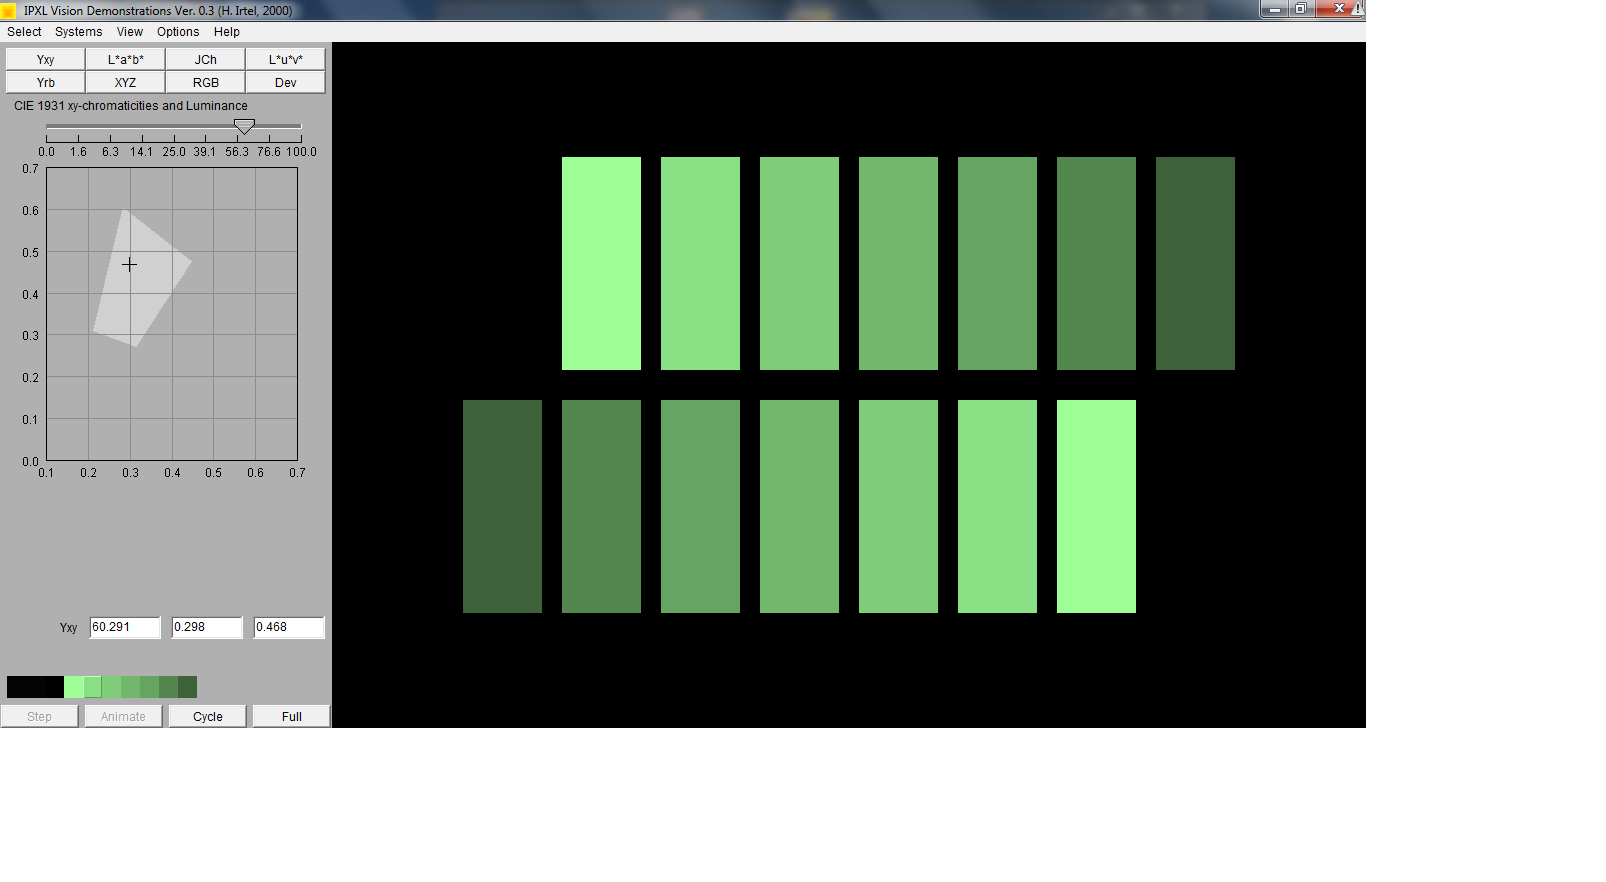
\includegraphics[width=\textwidth]{images/A5_Helligkeit.png}
    \caption{Farbenreihe für Änderung in der Helligkeit}
    \label{fig:A5b}
\end{figure}
\begin{figure}[H]
    \centering
    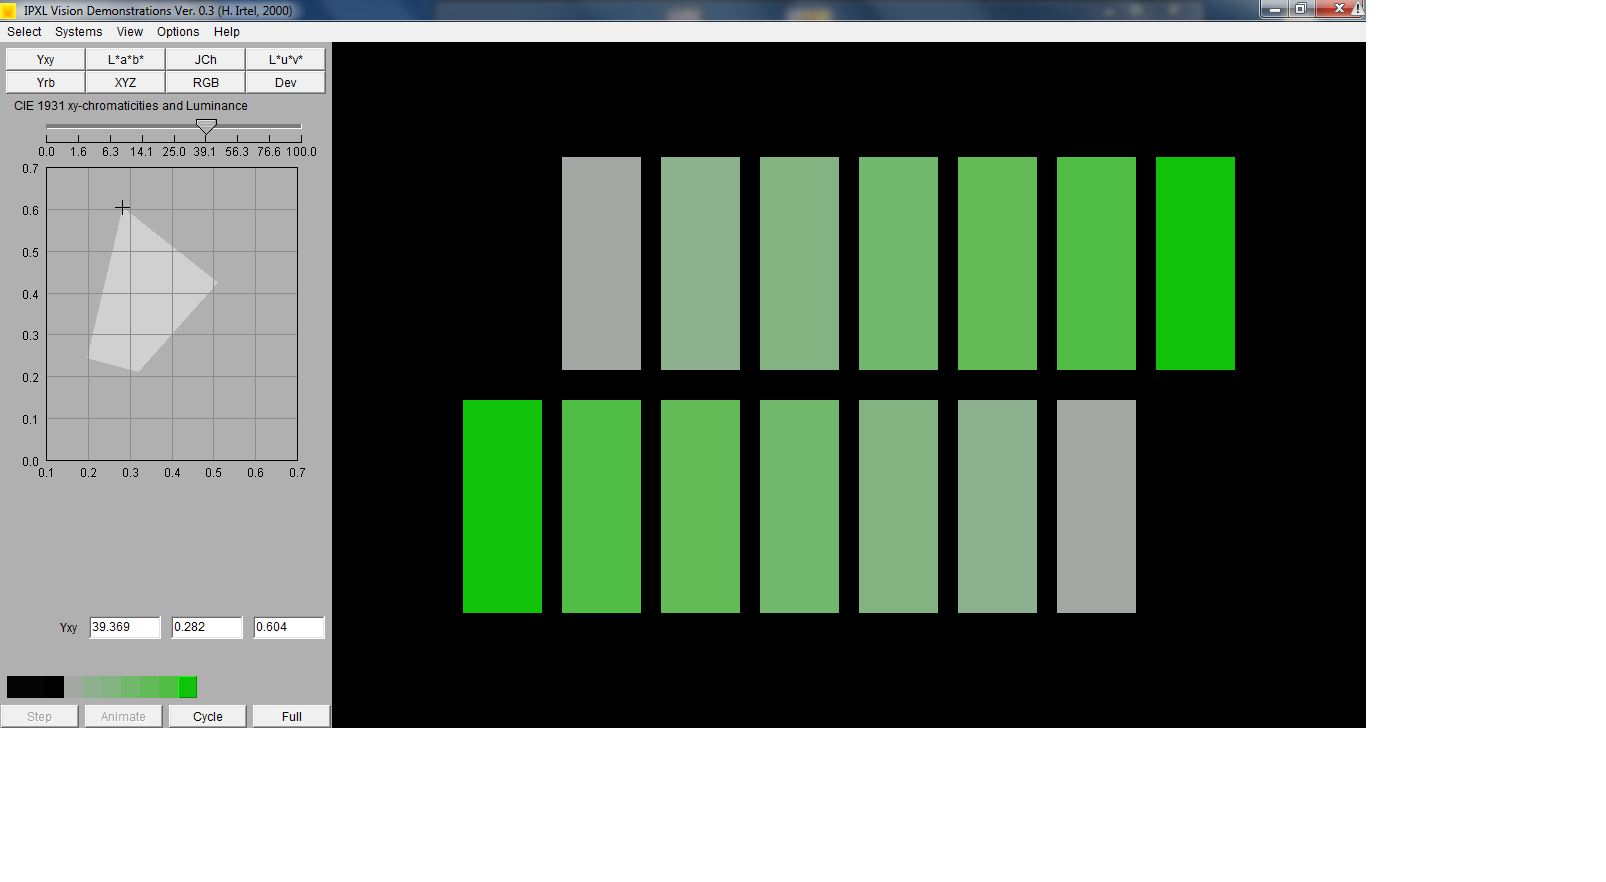
\includegraphics[width=\textwidth]{images/A5_Saettigung.png}
    \caption{Farbenreihe für Änderung in der Sättigung}
    \label{fig:A5c}
\end{figure}

\vspace{1.5\baselineskip}

\subsection{Farbmischung}
Die Farbmischung für das erste Farbenpaar ist in Abbildung \ref{fig:A6a} dargestellt. Die Farbmischung für das zweite Farbenpaar ist in Abbildung \ref{fig:A6b} dargestellt.
\begin{figure}[H]
    \centering
    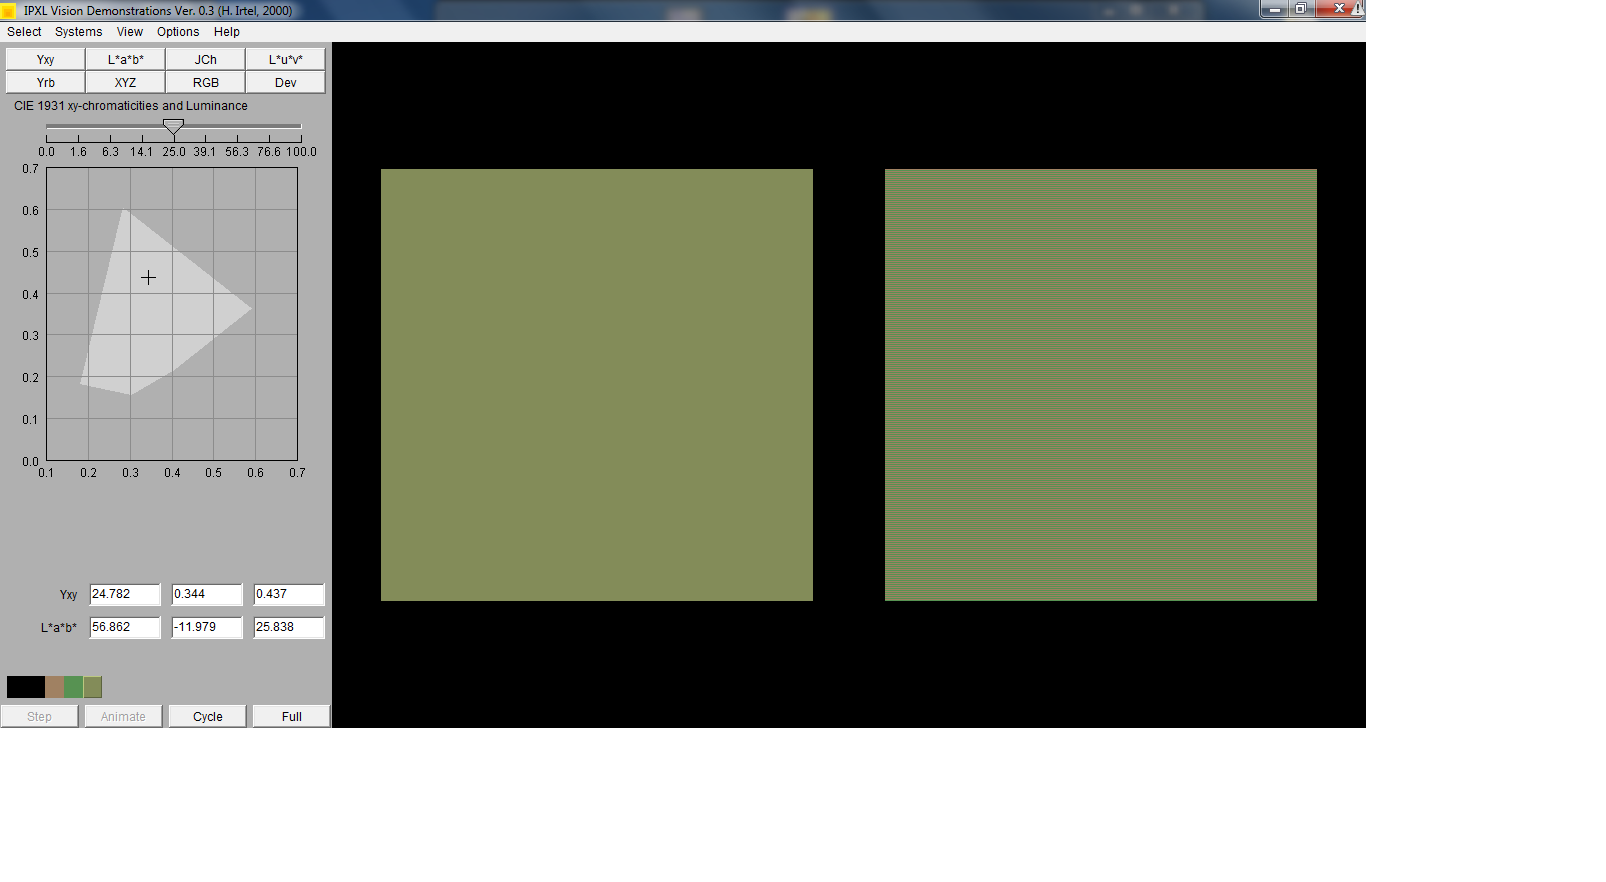
\includegraphics[width=\textwidth]{images/A6_Farbpaar1.png}
    \caption{Farbmischung für das erste Farbenpaar}
    \label{fig:A6a}
\end{figure}
\begin{figure}[H]
    \centering
    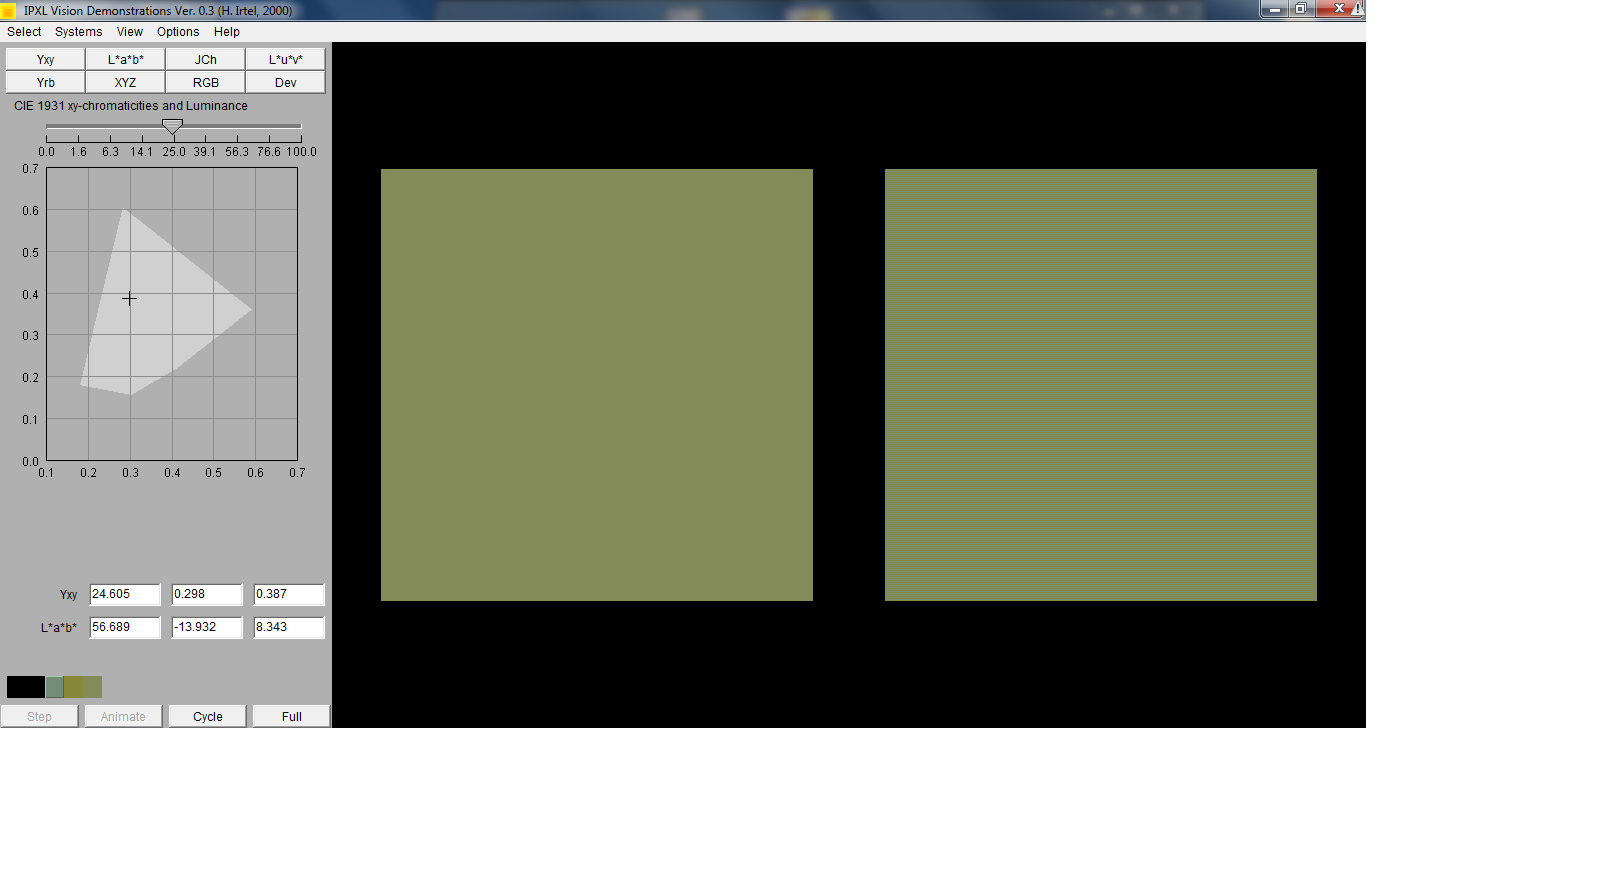
\includegraphics[width=\textwidth]{images/A6_Farbpaar2.png}
    \caption{Farbmischung für das zweite Farbenpaar}
    \label{fig:A6b}
\end{figure}

\subsection{Simultaner Farbkontrast}
Wenn die inneren Vierecke beide von Schwarz umgeben waren, schienen sie den gleichen Farbton zu haben. Wenn die inneren Vierecke von farbigen Vierecken umgeben waren, schienen sie unterschiedliche Farbtöne zu haben. Außerdem schien der Übergang der Vierecke links deutlich kontrastärmer.\\
Besonders starke Unterschiede wurden für folgende Farbkombination beobachtet:\\
Für die inneren Vierecke war der Farbton ein blasses, helles Rot. Der Farbton für das linke äußere Viereck war ein helles Grün, für das rechte äußere Viereck ein dunkles sattes Grün.
\begin{figure}[H]
    \centering
    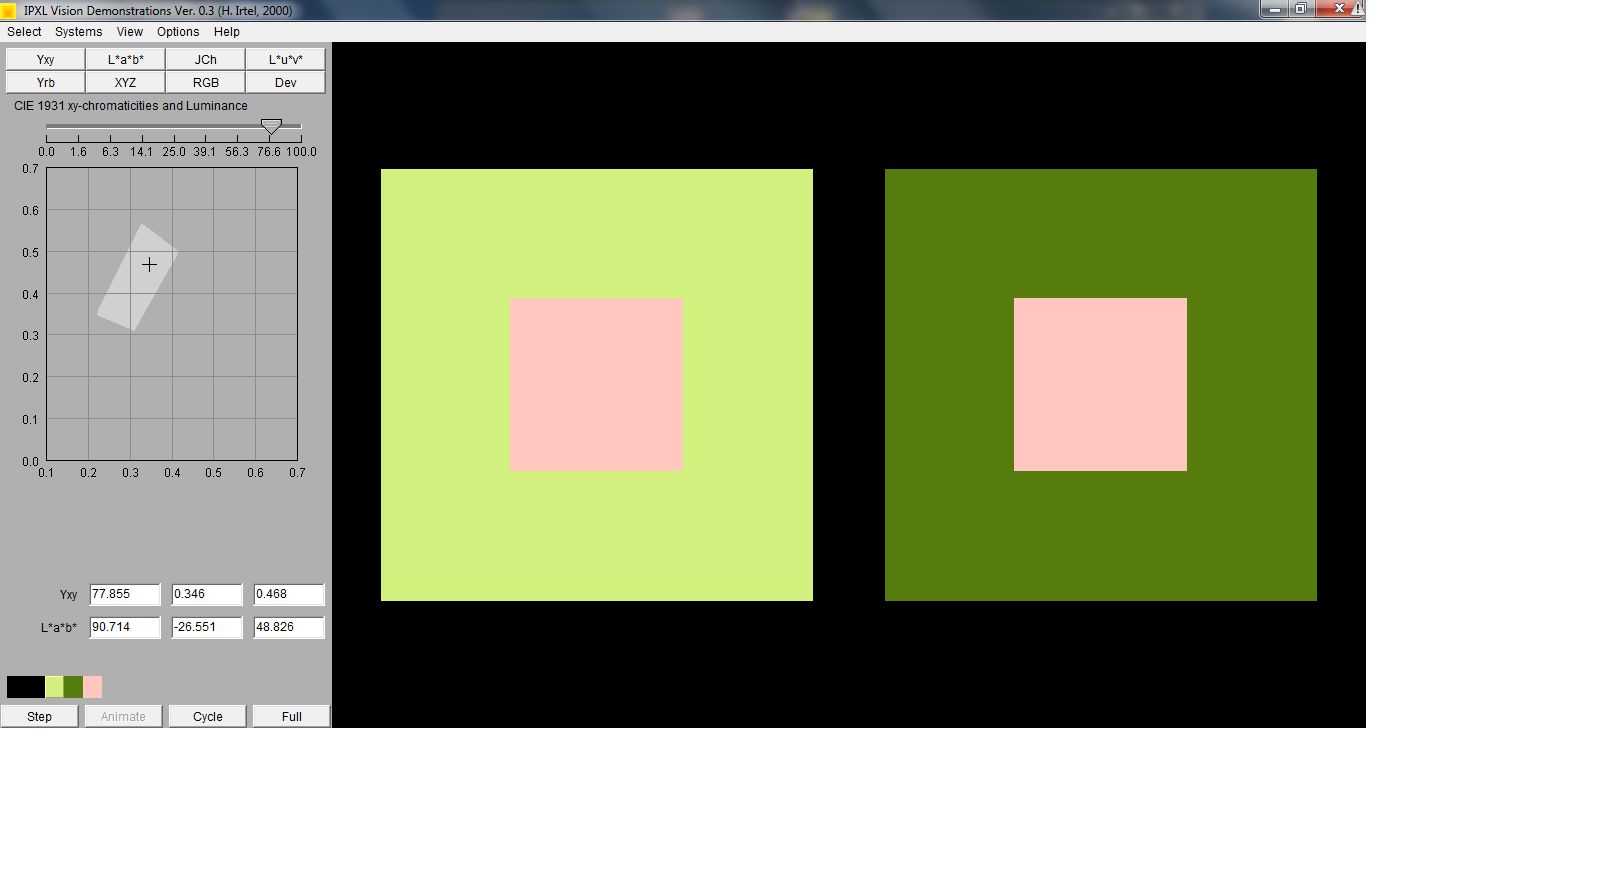
\includegraphics[width=\textwidth]{images/A7.png}
    \caption{Die blassrosanen inneren Vierecke erscheinen unterschiedlich.}
    \label{fig:A7}
\end{figure}

\subsection{Sukzessiver Farbkontrast}
Aftereffects and Opponent Colors:\\
Beim Nachbild erschien das gelbe Viereck dunkelblau, das blaue Viereck blassgelb, das grüne Viereck magenta, und das rote Viereck cyanfarben.\\
Induction:\\
Die rote Umrandung erschien cyanfarben. Der weiße Punkt erschien rot.\\
Desaturation:\\
Die linke Hälfte erschien in einem weniger kräftigen Gelb.\\
Hypersaturation:\\
Die drei ineinander geschachtelten Dreiecke erschienen in unterschiedlich hellen Gelbtönen (innen am hellsten, außen am dunkelsten).


%%
%%
%% Kapitel 4: Diskussion
%%
%%

\newpage
\section{Diskussion}

 \subsection{Farbenkreis}
Viele der ausgeführten Experimente waren eher von subjektiver und intuitiver Wahrnehmung geprägt. Besonders in diesem Experiment haben wir den Farbenkreis gänzlich über unser eigenes Farbempfinden und der Richtigkeit der Anordnung von Farben erstellt. 

 \subsection{Farbmischung I}
 
Hier konnte demonstriert werden, wie z.B. bei Monitoren und Fernseher durch verschiedene Farmmischungen der Grundfarben Rot, Gelb und Grün (RGB) unser Auge überlistet wird. Bei diesem Phänomen spricht man von der additiven Farbmischung und bei dem Menschen ist das Farbsehen durch den gleichen Effekt der drei Zapfentypen (S-, M-, L-Zapfen) im Auge geprägt. Dieser tritt auf wenn einem Farbeindruck jeweils ein anderer Farbreiz hinzugefügt wird. Da die additive Farmischung im Aufge und Gehirn stattfindet, spricht man hier auch von der physiologischen Farbmischung.

 \subsection{Farbintensität}
 Hier wurde gezeigt, wie wir als Menschen Farben je nach Werteverteilung bei Farbton, Sättigung und Helligkeit/Intesität wahrnehmen. Hierzu haben wir uns bei dem Experiment in einem Farbraum bewegen können, um eine Relation zwischen der menschlichen Farbwahrnehmung und den physikalischen Ursachen des Farbreizes herstellen zu können.

%% \subsection{Farbenreihe}
%% Da gibts eigentlich nix zu diskutieren
\subsection{Farbmischung}
Metamerie ist das Konzept, dass durch die enge räumliche Anordnung von mehreren Farben der Eindruck einer Vergleichsfarbe vermittelt wird. Dies ist möglich, da unser menschliches Auge nur drei verschiedene Rezeptoren (Zapfen) für unterschiedliche Wellenlänge enthält. Ein Farbton einer Wellenlänge erregt diese Zapfen auf die gleiche Art und Weise wie es metamere Farbtöne tun.
\subsection{Simultaner Farbkontrast}
Beim linken Viereckpaar ist die laterale Inhibition schwächer, da der Helligkeitsunterschied nicht so stark ist wie beim rechten Viereckspaar. Die Kanten erscheinen also weniger kontrastreich.
\subsection{Sukzessiver Farbkontrast}
Durch das lange fixieren der farbigen Objekte ermüden die Sehrezeptoren, die darauf fixiert sind und die Wellenlänge der Objektfarbe absorbieren. Konkret wird hier an den Rezeptoren Rhodopsin verbraucht, das sich nur allmählich wieder bildet.\\
Nach dem Übergang zwischen den Bildern feuern nun die Rezeptoren, deren Rhodopsin verbraucht ist nicht mehr. Es werden nur noch Signale an den Rezeptoren ausgesandt, die das Komplement der beobachteten Farbe wahrnehmen.
\printbibliography

\end{document}